\documentclass[a4paper,11pt]{article}
\usepackage[utf8]{inputenc}
\usepackage[T1]{fontenc}
\usepackage{lmodern}
\usepackage{subcaption}
\usepackage[siunitx]{circuitikz}
\usepackage{longtable}
\usepackage{titlesec}
\usepackage{graphicx}
\usepackage{amsmath}
\usepackage{float}
\usepackage[margin=2cm]{geometry}
\usepackage[justification=centering]{caption}
\DeclareGraphicsExtensions{.png}

\titleformat*{\section}{\sffamily\LARGE\bfseries}
\titleformat*{\subsection}{\sffamily\Large\bfseries}
\titleformat*{\subsubsection}{\sffamily\large\bfseries}

\begin{document}
\section*{Bauelementegleichungen}
\subsection*{Diode}
\subsubsection*{Diodenkennlinie:}
\[\boxed{I_D=I_S\left(e^{\frac{U_D}{U_T}}-1\right)}\]
Gilt für $U_D > 0V$. Wenn $U_D \leq 0V$, dann ist der Strom (idealisiert) $I_D = 0A$.

\subsection*{MOSFET}
\subsubsection*{Sperrbereich:}
\[\boxed{I_{Dn/p} = 0}\] 
wenn $ U_{GSn}-U_{Tn} \leq 0$ beim n-MOSFET\\
wenn $ U_{GSp}-U_{Tp} \geq 0$ beim p-MOSFET

\subsubsection*{Widerstandsbereich:}
\[\boxed{I_{Dn/p} = \pm\beta_{n/p}\left[(U_{GSn/p}-U_{Tn/p}) U_{DSn/p}-\dfrac{U_{DSn/p}^2}{2}\right](1\pm\lambda_{n/p}\ U_{DSn/p})}\] 
wenn $0<U_{DSn}<U_{GSn}-U_{Tn}$ und $\lambda_n>0$ beim n-MOSFET (+)\\
wenn $U_{GSp}-U_{Tp}<U_{DSp}<0$ und $\lambda_p>0$ beim p-MOSFET (-)

\subsubsection*{Sättigungsbereich:}
\[\boxed{I_{Dn/p}=\pm\dfrac{1}{2}\beta_{n/p}\left(U_{GSn/p}-U_{Tn/p}\right)^2\ (1\pm\lambda_{n/p}\ U_{DSn/p})}\]
wenn $U_{DSn}\geq U_{GSn}-U_{Tn}>0$ und $\lambda_n>0$ beim n-MOSFET (+)\\
wenn $U_{DSp}\leq U_{GSp}-U_{Tp}<0$ und $\lambda_p>0$ beim p-MOSFET (-)

\subsubsection*{3D-Plot n-Kanal-MOSFET}
\begin{figure}[H]
\begin{subfigure}{0.32\textwidth}
	\begin{center}
		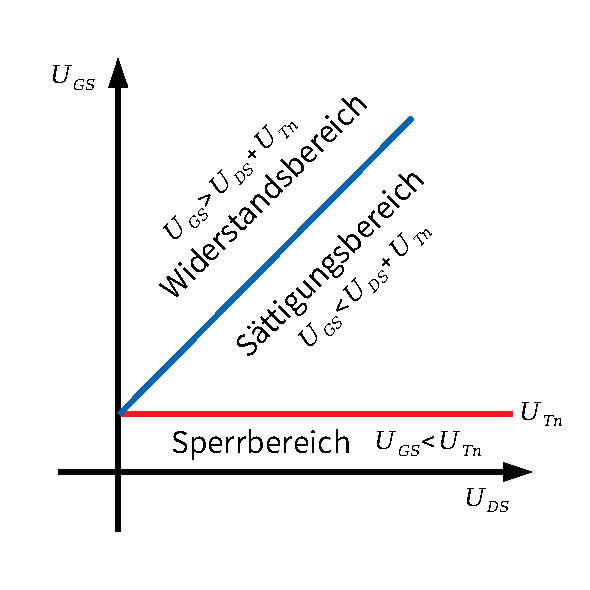
\includegraphics[width=\textwidth]{img/nmosfet_operationmodes.pdf}
	\end{center}
\end{subfigure}
\begin{subfigure}{0.67\textwidth}
	\begin{center}
		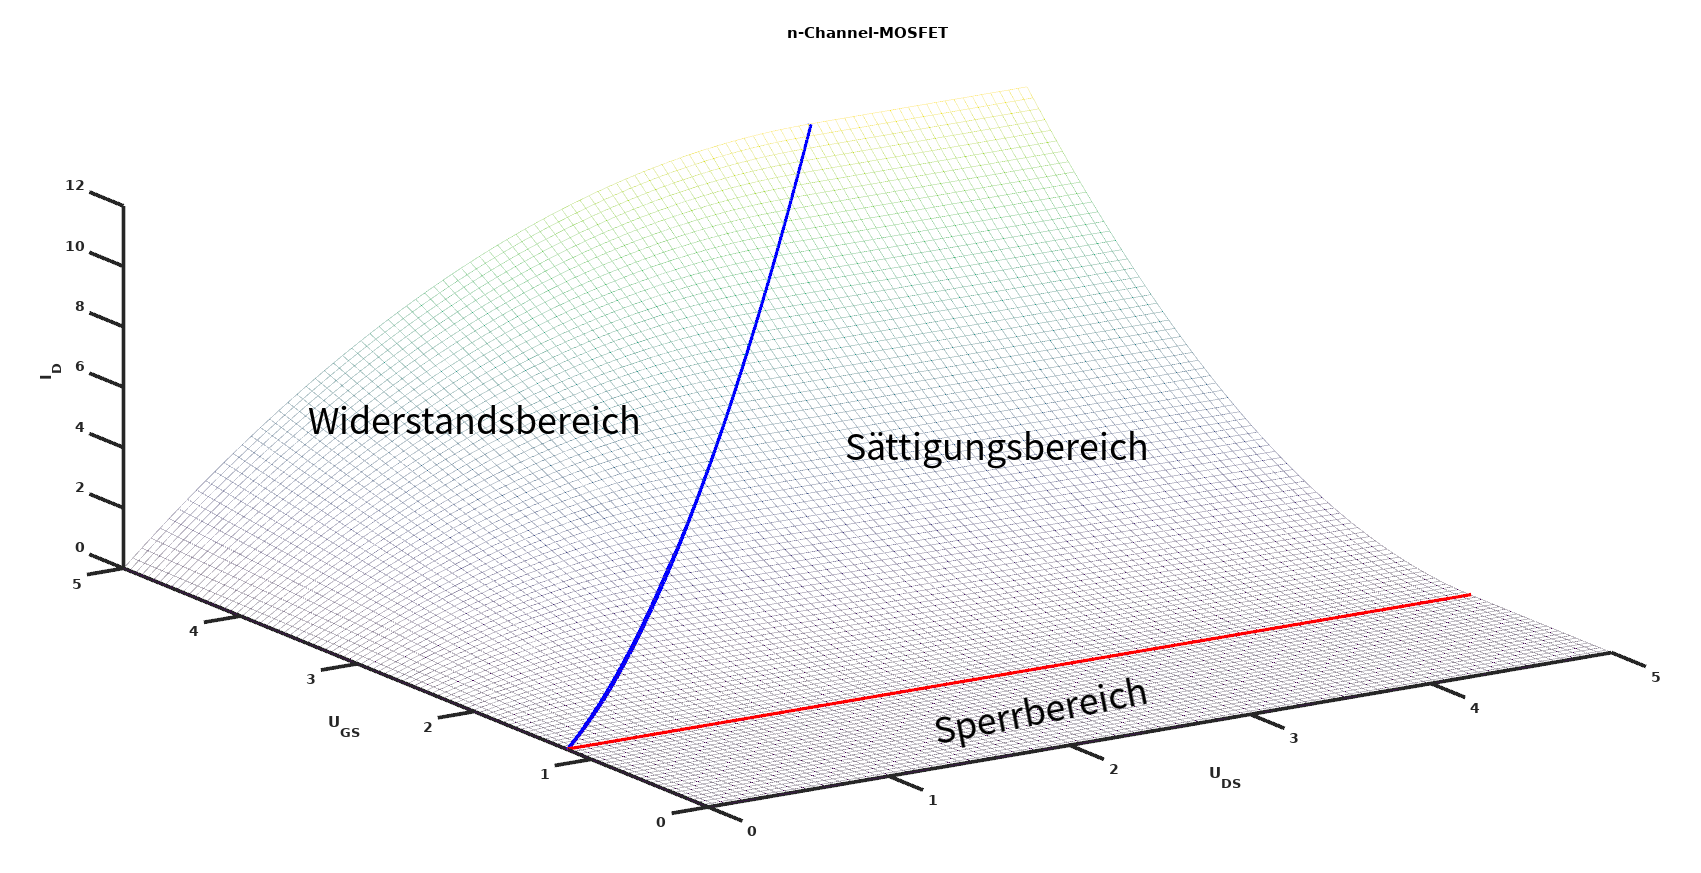
\includegraphics[width=\textwidth]{img/nmosfet_3dplot}
	\end{center}
\end{subfigure}
\end{figure}

\subsubsection*{3D-Plot p-Kanal-MOSFET}
\begin{figure}[H]
\begin{subfigure}{0.32\textwidth}
	\begin{center}
		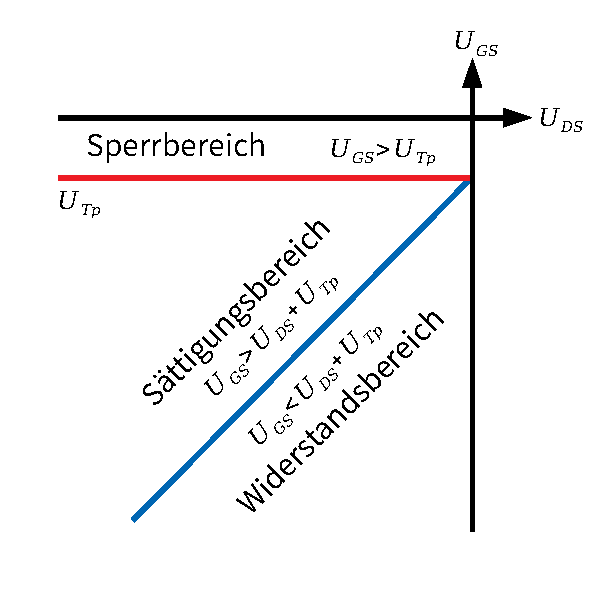
\includegraphics[width=\textwidth]{img/pmosfet_operationmodes.pdf}
	\end{center}
\end{subfigure}
\begin{subfigure}{0.67\textwidth}
	\begin{center}
		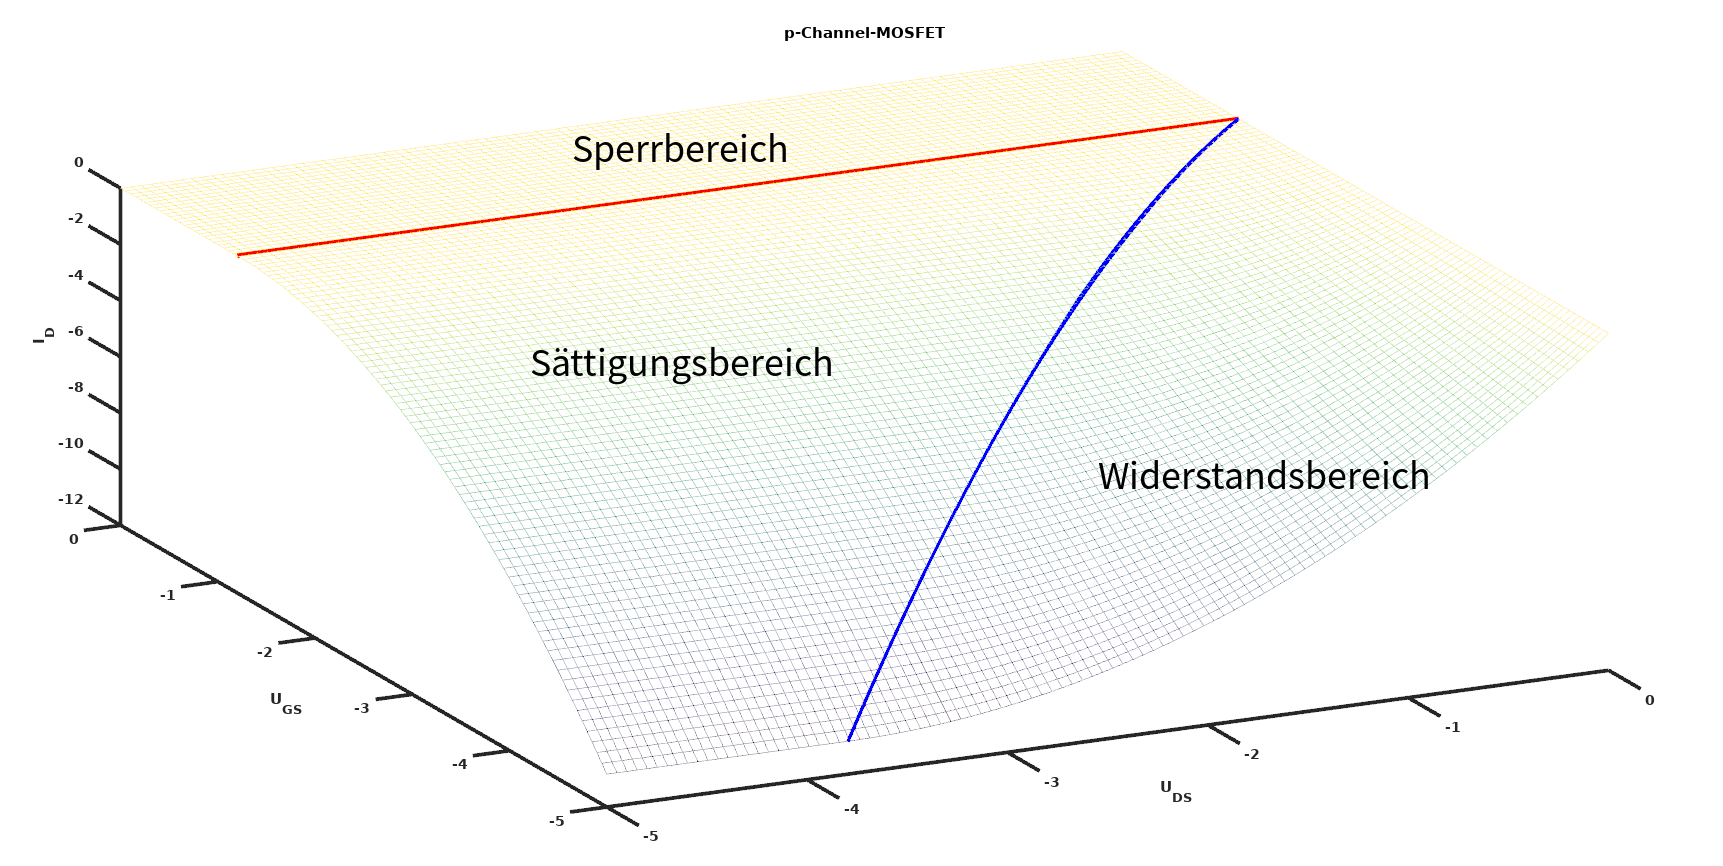
\includegraphics[width=\textwidth]{img/pmosfet_3dplot}
	\end{center}
\end{subfigure}
\end{figure}

\section*{Prozessparameter}
\subsection*{Prozessverstärkungsfaktor (\textit{transconductance coefficient})}
\[
	\boxed { \quad \beta_n = k_n ~ \frac{W}{L_{eff}} \quad } \qquad \boxed { \quad \beta_p = k_p ~ \frac{W}{L_{eff}} \quad }
\]

\[
	k_n = \mu_n ~ C_{ox}' = \frac{\mu_n ~ \varepsilon_0 ~ \varepsilon_{SiO_2}}{d_{ox}} \stackrel{typ.}{=} 30 \ldots 200 ~ \frac{\mu A}{V^2}
\]

\[
	k_p = \mu_p ~ C_{ox}' = \frac{\mu_p ~ \varepsilon_0 ~ \varepsilon_{SiO_2}}{d_{ox}} \stackrel{typ.}{=} 15 \ldots 100 ~ \frac{\mu A}{V^2}
\]

\section*{Parasitäre Kapazitäten}
Mit $C_G = C_{ox}' ~ W ~ L$:

\begin{center}
\begin{tabular}{r l}
	$C_{GS} = C_G$ & Gate-Source-Kapazität \\
	$C_j = \frac{2}{3} ~ C_G$ & Drain/Source-Bulk-Sperrschichtkapazität (junction) \\
	$C_{GD} = \frac{2}{3} ~ C_G$ & Gate-Drain-Kapazität
\end{tabular}
\end{center}

\section*{Störabstände (\textit{noise margins})}
\begin{figure}[H]
\begin{center}
	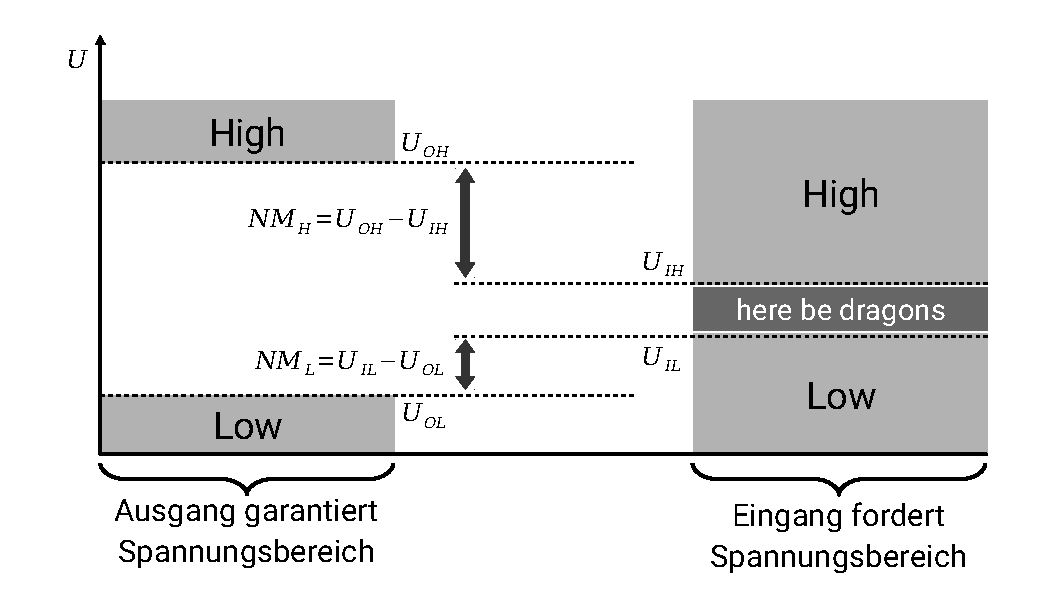
\includegraphics[width=0.9\textwidth]{img/noisemargin.pdf}
\end{center}
\end{figure}

\section*{Dimensionierung und Gateweiten}
\subsection*{Effektive Gateweite bestimmen}
\begin{itemize}
	\item Bestimmen, welche FETs im gegebenen Fall (z.B. Worst-Case) leiten
	\item Nicht leitende FETs erhalten Gateweite 0, andere erhalten physikalische Gateweite
	\item Mit Gateweiten (nächerungsweise) wie mit Leitwerten rechnen und Schrittweise zusammenfassen
	\[
		\boxed{\quad \mathrm{Reihenschaltung:} \quad W_{ges} = W_1 + W_2 + \ldots \qquad \mathrm{Parallelschaltung:} \quad W_{\parallel} = \frac{1}{\frac{1}{W_1} + \frac{1}{W_2} + \frac{1}{\ldots}} \quad}
	\]
	\item Effektive Gateweite ist Ergebnis für die gesamte betrachete Schaltung (z.B. n-Kanal-Zweig)
\end{itemize}

\subsection*{Dimensionierung auf symmetrische Schaltflanken im Worst-Case}
\begin{itemize}
\item Effektive Gateweite des schon bekannten Zweiges bestimmen
\item Für symmetrische Schaltflanken muss gelten:
\[
\boxed{\quad W_{P, \mathrm{eff}} \overset{!}{=} \beta_R ~ W_{N, \mathrm{eff}} \overset{\mathrm{typ}.}{=} 2 ~ W_{N, \mathrm{eff}} \quad}
\]
\item Längste MOSFET-Kette im zu dimensionierenden Kanalzweig mit Länge $N$ erhält $W = \frac{W_{\mathrm{eff}}}{N}$
\item Parallele Kettenschaltungen auf gleiche effektive Gateweite dimensionieren
\end{itemize}

\section*{Verzögerungszeiten}
\subsection*{Laden / Entladen einer Kapazität}
\[
	i(t) = -C_L ~ \frac{\mathrm du_c(t)}{\mathrm dt}
\]

Problem: Finde $t$, stelle also um:
\[
	\mathrm dt = - \frac{C_L}{i(t)} ~ \mathrm du_c
\]

Wobei $i(t)$ durch die Gleichung des entsprechendes MOSFETs bestimmt wird, d.h. nur von $u_c$ abhängt. Die Gesamtzeit ergibt sich dann durch Integration:
\[
	t_{charge} = - \int_{U_{start}}^{U_{end}} \frac{C_L}{I_{DS}(u_c)} ~ \mathrm du_c
\]

In der Regel muss dabei eine Fallunterscheidung für die verschiedenen Betriebsbereiche des MOSFETs getroffen werden mit dazugehörigem $I_{DS}$.

Wichtig: Als Endwert sollte nicht die vollständige Umladung (also $U_{DD}$ oder $0V$) verwendet werden, da dieser Wert mathematisch nie erreicht wird.

\subsubsection*{Kapazität über NMOS entladen}

\begin{figure}[H]
\centering
\begin{subfigure}{.35\textwidth}
	\centering
	\begin{circuitikz}[european, scale=0.7]
		\draw
			(0,0) node[nigfetebulk](nmos1){}
			(nmos1.S) to node[ground]{} (0, -1)
			(nmos1.D) to ++(0, 0.5) to [short,i<=$i(t)$] ++(1.5, 0) to [C,l^=$C_L$] (1.5, -1) to node[ground]{} (1.5, -1)
			(nmos1.G) to [short, -o] ++(-1.5, 0) node[label={[font=\footnotesize]above:$U_G(t) = U_{DD}$}]{}
		;
	\end{circuitikz}
\end{subfigure}
\begin{subfigure}{.49\textwidth}
	\begin{tabular}{r l}
		\textbf{Startspannung} & $U_{start} = U_{DD}$ \\
		\textbf{Zielspannung} & $U_{end} = 0.1 ~ U_{DD}$ \\
		\textbf{Threshold-Spannung} & $U_{Tn} = 0.2 ~ U_{DD}$ \\
		\textbf{Kanallängenmodulation} & vernachlässigt, $\lambda = 0$
	\end{tabular}
\end{subfigure}
\end{figure}

Abfallzeit:
\[
	\boxed{ \quad t_{HL} \approx 4 ~ \frac{C_L}{\beta_n ~ U_{DD}} \quad }
\]

\subsubsection*{Kapazität über PMOS laden}

\begin{figure}[H]
\centering
\begin{subfigure}{.35\textwidth}
	\centering
	\begin{circuitikz}[european, scale=0.7]
		\draw
			(0,0) node[pigfetebulk, rotate=90](pmos1){}
			(pmos1.G) to [short] ++(0, -1) node[ground,label={[font=\footnotesize]left:$U_G(t) = 0V$}]{}
			(pmos1.S) to [short, -o] ++(-1, 0) node[label={[font=\footnotesize]above:$U_{DD}$}]{}
			(pmos1.D) to [short,i<=$i(t)$] ++(1, 0) to [C,l^=$C_L$] ++(0,-2.4) node[ground]{}
		;
	\end{circuitikz}
	\caption*{Beachte: $i(t) < 0$}
\end{subfigure}
\begin{subfigure}{.49\textwidth}
	\begin{tabular}{r l}
		\textbf{Startspannung} & $U_{start} = 0V$ \\
		\textbf{Zielspannung} & $U_{end} = 0.9 ~ U_{DD}$ \\
		\textbf{Threshold-Spannung} & $U_{Tp} = -0.2 ~ U_{DD}$ \\
		\textbf{Kanallängenmodulation} & vernachlässigt, $\lambda = 0$
	\end{tabular}
\end{subfigure}
\end{figure}

Anstiegszeit:
\[
	\boxed{ \quad t_{LH} \approx 4 ~ \frac{C_L}{\beta_p ~ U_{DD}} \quad }
\]

\subsubsection*{Kapazität über NMOS laden}

\begin{figure}[H]
\centering
\begin{subfigure}{.35\textwidth}
	\centering
	\begin{circuitikz}[european, scale=0.7]
		\draw
			(0,0) node[nigfetebulk, rotate=90](nmos1){}
			(nmos1.G) to [short,-o] ++(-2.5, 0) node[label={[font=\footnotesize]above:$U_G(t) = U_{DD}$}]{}
			(nmos1.D) to [short, -o] ++(-1, 0) node[label={[font=\footnotesize]above:$U_{DD}$}]{}
			(nmos1.S) to [short,i<=$i(t)$] ++(1, 0) to [C,l^=$C_L$] ++(0,-2.4) node[ground]{}
		;
	\end{circuitikz}
	\caption*{Beachte: $i(t) < 0$}
\end{subfigure}
\begin{subfigure}{.49\textwidth}
	\begin{tabular}{r l}
		\textbf{Startspannung} & $U_{start} = 0V$ \\
		\textbf{Zielspannung} & $U_{end} = 0.9 ~ (U_{DD} - U_{Tn})$ \\
		\textbf{Threshold-Spannung} & egal (immer Sättigungsbereich) \\
		\textbf{Kanallängenmodulation} & vernachlässigt, $\lambda = 0$
	\end{tabular}
\end{subfigure}
\end{figure}

Anstiegszeit:
\[
	\boxed{ \quad t_{LH} \approx 18 ~ \frac{C_L}{\beta_n ~ (U_{DD} - U_{Tn})} \quad }
\]

\subsubsection*{Über NMOS geladene Kapazität wieder mit NMOS entladen}

\begin{figure}[H]
\centering
\begin{subfigure}{.35\textwidth}
	\centering
	\begin{circuitikz}[european, scale=0.7]
		\draw
			(0,0) node[nigfetebulk](nmos1){}
			(nmos1.S) to node[ground]{} (0, -1)
			(nmos1.D) to ++(0, 0.5) to [short,i<=$i(t)$] ++(1.5, 0) to [C,l^=$C_L$] (1.5, -1) to node[ground]{} (1.5, -1)
			(nmos1.G) to [short, -o] ++(-1.5, 0) node[label={[font=\footnotesize]above:$U_G(t) = U_{DD}$}]{}
		;
	\end{circuitikz}
\end{subfigure}
\begin{subfigure}{.49\textwidth}
	\begin{tabular}{r l}
		\textbf{Startspannung} & $U_{start} = U_{DD} - U_{Tn}$ (\textbf{!!!}) \\
		\textbf{Zielspannung} & $U_{end} = 0.1 ~ (U_{DD} - U_{Tn})$ \\
		\textbf{Threshold-Spannung} & egal (immer linearer Bereich) \\
		\textbf{Kanallängenmodulation} & vernachlässigt, $\lambda = 0$
	\end{tabular}
\end{subfigure}
\end{figure}

Abfallzeit:
\[
	\boxed{ \quad t_{HL} \approx 3 ~ \frac{C_L}{\beta_n ~ (U_{DD} - U_{Tn})} \quad }
\]

\subsection*{Durchschnittliche Verzögerungszeit $t_p$}
Die Durchschnittliche Verzögerungszeit $t_p$ gibt die durchschnittliche Zeit an, die verstreicht zwischen dem Moment, an dem das Eingangssignal den Schaltpunkt $50 \% ~ U_{DD}$ erreicht und dem Moment, an dem das Ausgangssignal ebenfalls den Schaltpunkt überstreicht. Es wird zwischen Anstiegs- und Abfallzeit gemittelt, $t_p = \frac{t_{pHL} + t_{pLH}}{2}$.

Sei Eingangssignal ideal (rechteckförmig) und Umladung erfolgt linear. Dann ist $50 \% ~ U_{DD}$ schon nach der Hälfte der Anstiegs- / Abfallzeit erreicht, d.h. $t_{pHL} = \frac{1}{2} ~ t_{HL}$, $t_{pLH} = \frac{1}{2} ~ t_{LH}$. Somit:
\[
	t_p = \frac{t_{HL} + t_{LH}}{4}
\]

Für den \textbf{CMOS-Inverter} oder Schaltungen mit äquivalenten Transistoren gilt bei symmetrischer Dimensionierung ($\beta_p = \beta_n$): Die Flanken sind symmetrisch und die Verzögerungszeit ist
\[
	\boxed{ \quad t_p \approx \frac{2 ~ C_L}{\beta_n ~ U_{DD}} \quad }
\]
\end{document}